\begin{flushleft}
Per determinare la radice della funzione data, abbiamo scritto il seguente script MatLab:
\lstinputlisting[language=Matlab]{cap_2/es8/es8.m}
Con risultato in output:
\newline
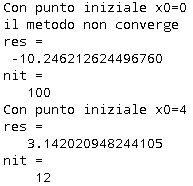
\includegraphics[width=150px]{cap_2/es8/es28.png}
\newline
Si può vedere che il metodo non converge per il punto iniziale $x0=0$, ma con punto iniziale diverso $x0=4$ il metodo converge. Questo significa che il metodo può convergere localmente. Dobbiamo quindi studiare la convergenza locale della funzione $f(x)$. Tale convergenza risulta essere garantita solo in un intorno della radice, in questo caso in un intorno di $\pi$. Essendo la funzione $f(x) = (x-\pi)\cdot e^{10\cdot x}$ la funzione di iterazione che definisce il metodo è determinata da:
\[
\Phi(x) = x-\frac{(x-\pi)\cdot e^{10\cdot x}}{e^{10\cdot x}\cdot (10\cdot x - 10 \cdot \pi + 1)} = x - \frac{(x-\pi)}{(10\cdot x - 10 \cdot \pi + 1)}
\]
Per convergere localmente si deve avere $\pi$ punto fisso della funzione di iterazione $\Phi(x)$. si ha infatti che:
\[
\Phi(\pi) = \pi - \frac{(\pi-\pi)}{(10\cdot \pi - 10 \cdot \pi + 1)} = \pi - 0 = \pi
\]
Questo conferma il fatto che la funzione $f(x)$ è convergente localmente in un intorno di $\pi$, confermando i risultati ottenuti dallo script precedente.
\end{flushleft}